2.  \begin{figure}[ht!]
\center{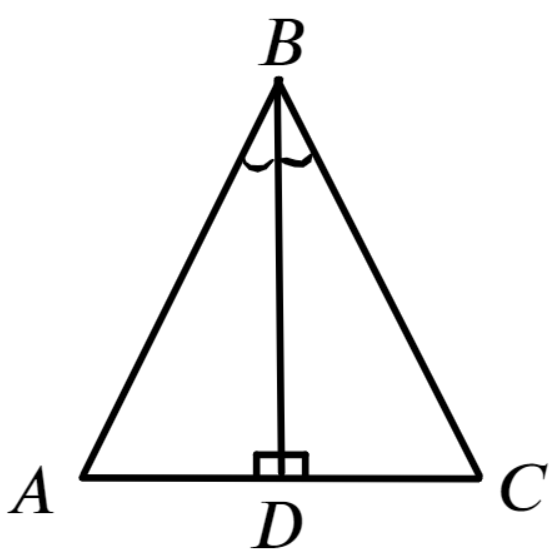
\includegraphics[scale=0.35]{g2.png}}
\end{figure}\\
$\left.\begin{array}{l}\angle ABD=\angle CBD\text{ т.к. }BD\text{ биссектриса,}\\
\angle ADB=\angle CDB=90^\circ \text{ т.к. }BD\text{ высота,}\\
BD - \text{ общая.}   \end{array}\right\}\Rightarrow
\Delta ADB=\Delta CDB\text{ по II признаку }\Rightarrow BA=BC\text{ ч.т.д.} $\\
